\section{Selection t-SNE Visualizations}
\label{app:selection-tsne}

We visualize the selected subsets in a shared low-dimensional embedding space. These plots are qualitative: the t-SNE coordinates~\citep{van2008visualizing} are computed from lightweight image proxy embeddings and are used only for visualization. Gray points denote source candidates, and colored points denote the subset selected by each method.

The ratio-$0.10$ plots in Figures~\ref{fig:tsne-r01-coco} and~\ref{fig:tsne-r01-kitti} show the selected subsets for COCO and KITTI. The ratio-$0.05$ COCO pose-estimation plots in Figures~\ref{fig:tsne-r005-coco} and~\ref{fig:tsne-overlay-r005-coco} examine the selection under an aggressive source budget ($n=1{,}000$, $5\%$ of the candidate pool), directly matching the constrained-budget retraining evaluations in Table~\ref{tab:constrained-source-budget}. The overlay figure makes the spatial separation between \model and representative active-learning baselines straightforward to inspect.

The visual pattern should be interpreted in light of the selection score in Section~\ref{subsec:slice-enrichment}. \model is not designed to be a uniformly spread coreset in the t-SNE plane. It behaves more like an attribute-conditioned real-source search: the selected images are related to the repair attributes, but they are spread across more diverse backgrounds, classes, and nearby contexts. The rarity term $\textcolor{colorR}{R_{i,a}}$ intentionally gives higher priority to source examples whose attribute values are rare within their class, so \model can place more mass on peripheral or less common regions of the proxy embedding. These peripheral selections are consistent with the intended rare-case behavior, although the t-SNE plot alone should be read only as a qualitative diagnostic. The penalty term $\textcolor{colorP}{P_{i,a}}$ reduces the priority of attribute values already supplied by the generated pool, so the selected source points are encouraged to complement the synthetic repair data instead of repeating it. Finally, the soft class-balance correction $\textcolor{colorC}{C_c^{(k)}}$ pulls the greedy selection away from a single high-scoring class or local region. The expected pattern is controlled non-uniformity: \model may put more mass on visually or semantically unusual regions than random, uncertainty, or pure coverage baselines while retaining cross-class coverage through the balance term.

The COCO overlay in Figure~\ref{fig:tsne-overlay-r005-coco} and facet panels in Figure~\ref{fig:tsne-r005-coco} illustrate this qualitative behavior under severe resource constraints. Under this $5\%$ budget, all generic active-learning selectors incur performance degradation (test AP between $0.5693$ and $0.5827$, relative to the pre-repair base of $0.5902$) because they either sample central mass broadly (Random and Stratified), concentrate tightly on ambiguous high-entropy clusters (Entropy and BADGE), or force extreme geometric dispersion along the perimeter (CoreSet) without targeting the diagnosed repair slice. In contrast, \model is the only method achieving positive repair (test AP $0.5969$, RER $+1.63\%$). Spatially, its selections concentrate on attribute-relevant subregions (clothing color brown and rainy weather) while deploying points across less frequent attribute combinations along the manifold periphery. Because t-SNE is only a two-dimensional proxy visualization, these plots should not be interpreted as standalone proof that shifting points improves downstream repair. They instead provide a qualitative sanity check that \model is not visibly collapsing onto the same region as the standard active-learning selectors.

% \begin{figure}[p]
% \centering
% \includegraphics[width=\linewidth]{figures/ratio0p1_selection_tsne/imagenet_controlnet_ratio0p1_selection_tsne.png}
% \caption{ImageNet ratio-$0.10$ selected subsets visualized on a shared source-image t-SNE embedding. Gray points show source candidates; colored points show the subset selected by each method.}
% \label{fig:tsne-r01-imagenet}
% \end{figure}

% \begin{figure}[p]
% \centering
% \includegraphics[width=\linewidth]{figures/ratio0p1_selection_tsne/celeba_redhair_brownskin_sademotion_ratio0p1_selection_tsne.png}
% \caption{CelebA ratio-$0.10$ selected subsets visualized on a shared source-image t-SNE embedding.}
% \label{fig:tsne-r01-celeba}
% \end{figure}

\begin{figure*}[p]
\centering
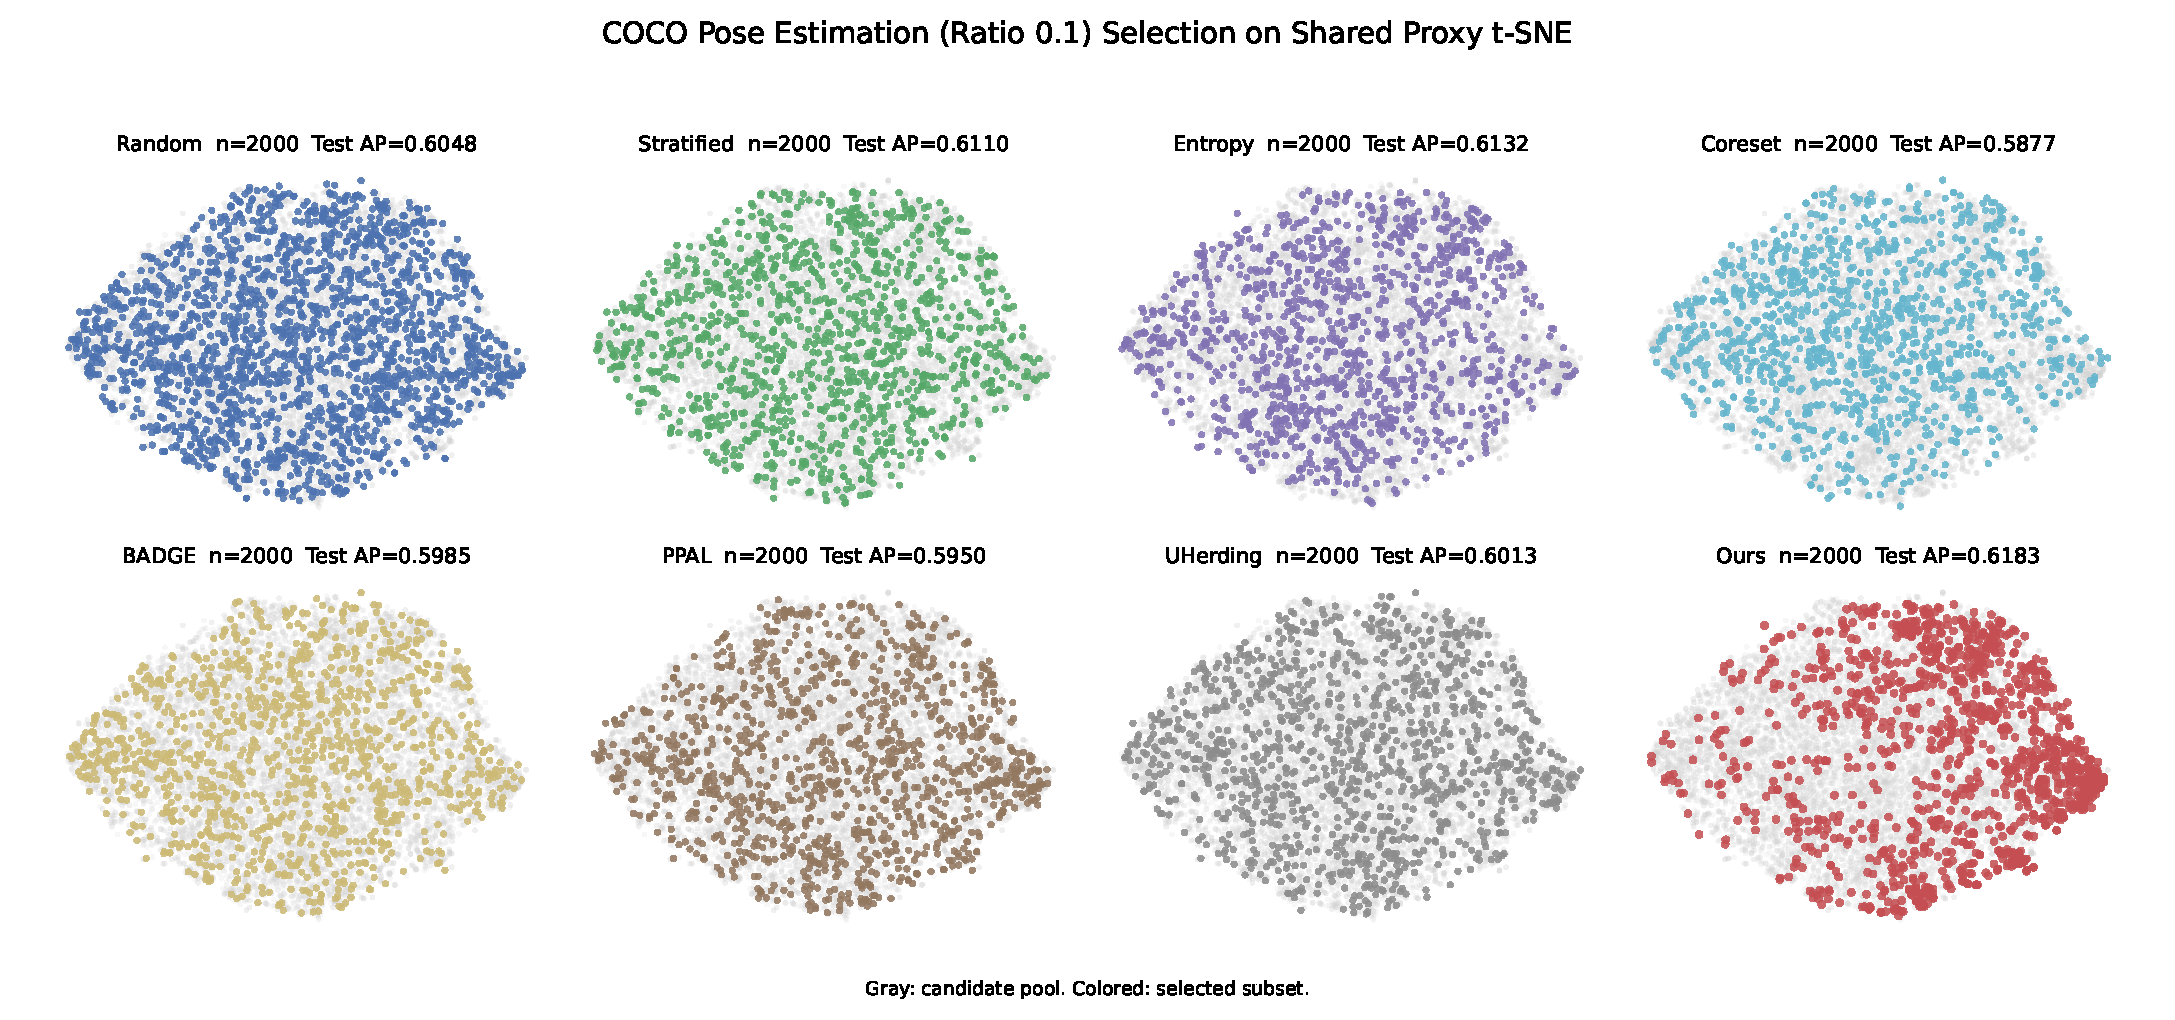
\includegraphics[width=\linewidth]{figures/ratio0p1_selection_tsne/coco_brown_rainy_ratio0p1_selection_tsne.pdf}
\caption{COCO pose-estimation ratio-$0.10$ selected subsets visualized on a shared source-image t-SNE embedding. Each method selects an identical source budget of $n=2{,}000$ training images from the $N=20{,}000$ candidate pool; for visual clarity, 12,000 randomly subsampled candidate points are displayed in the background.}
\label{fig:tsne-r01-coco}
\end{figure*}

\begin{figure*}[p]
\centering
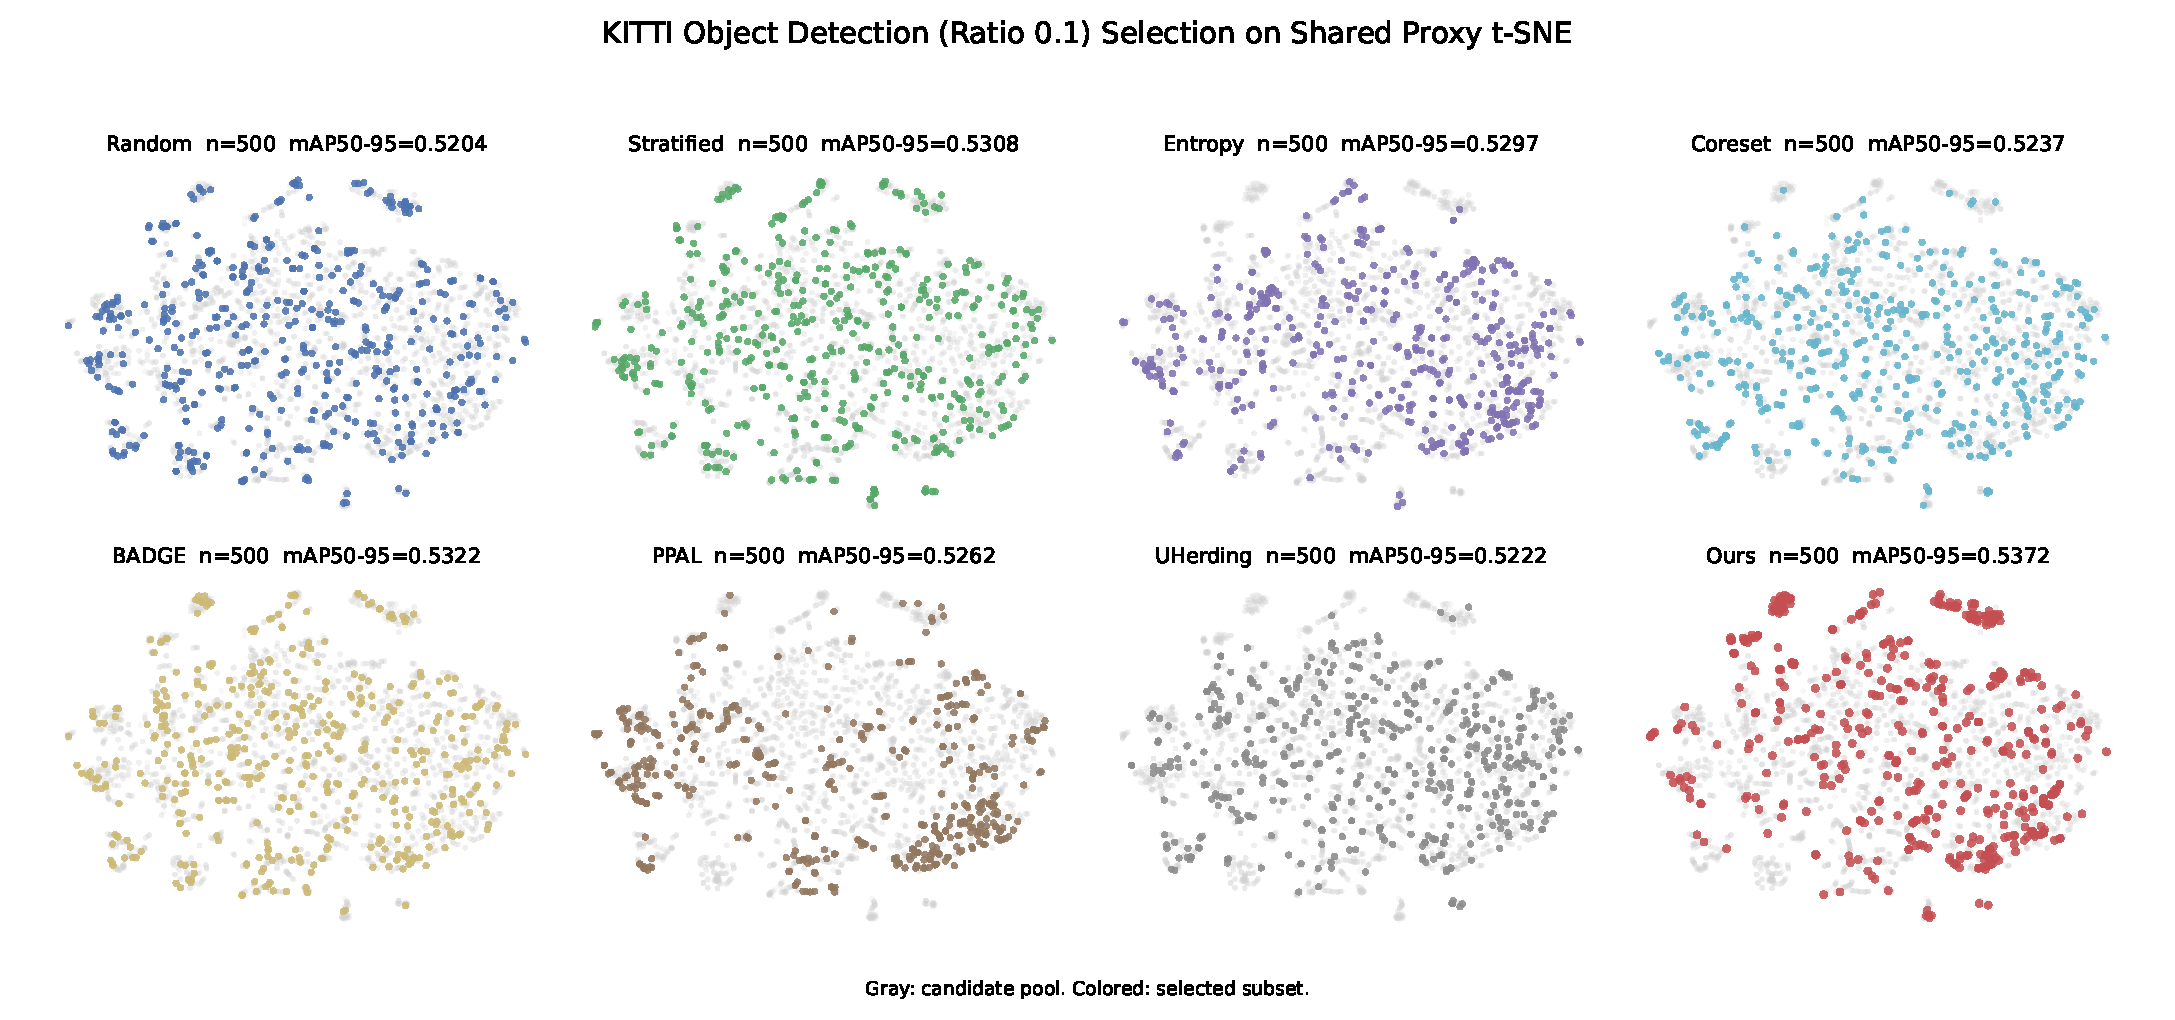
\includegraphics[width=\linewidth]{figures/ratio0p1_selection_tsne/kitti_red_cloudy_ratio0p1_selection_tsne.pdf}
\caption{KITTI object-detection ratio-$0.10$ selected subsets visualized on a shared source-image t-SNE embedding ($n=500$).}
\label{fig:tsne-r01-kitti}
\end{figure*}

% \begin{figure}[p]
% \centering
% 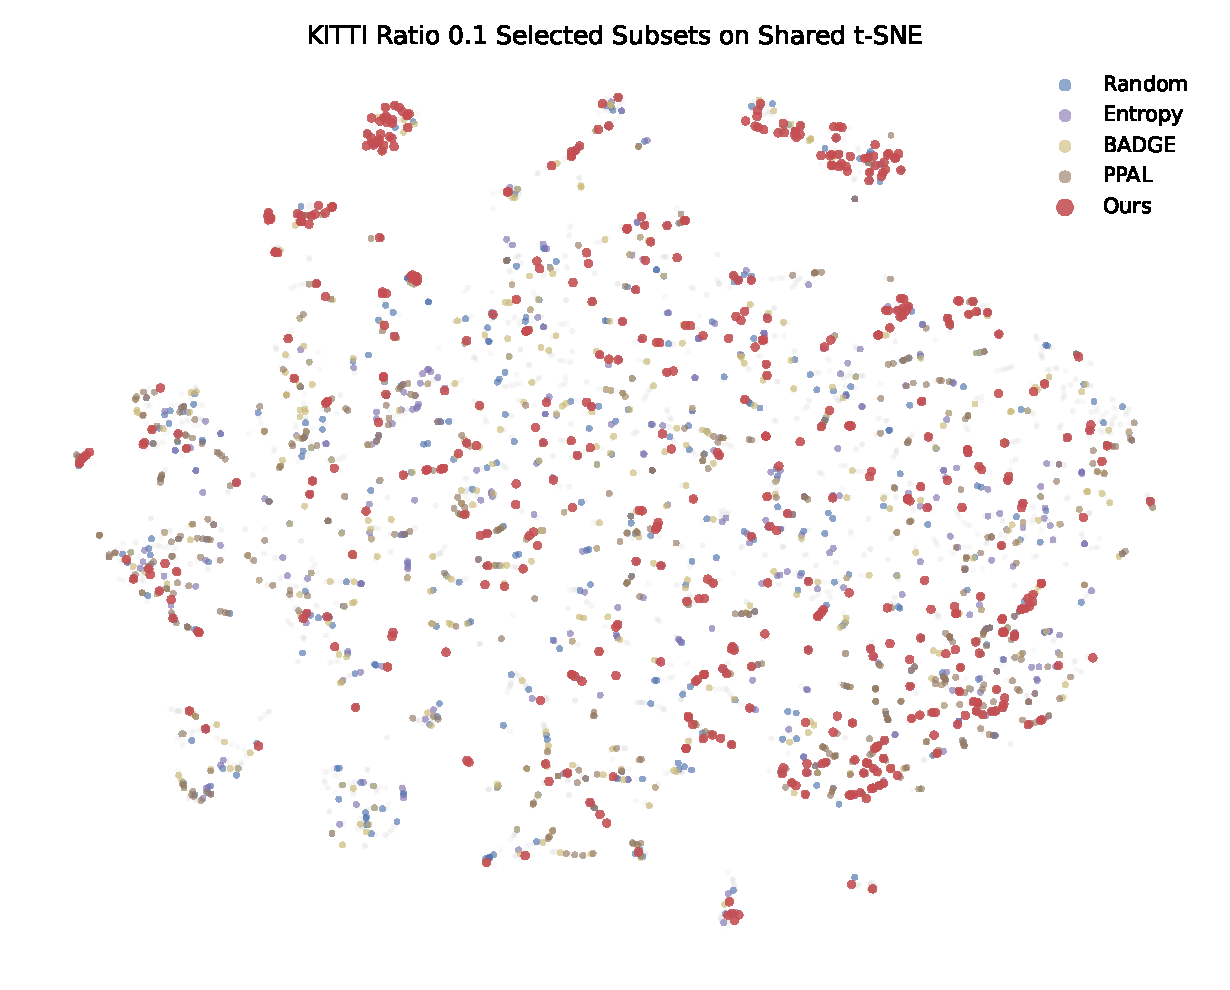
\includegraphics[width=0.86\linewidth]{figures/ratio0p1_selection_tsne/kitti_red_cloudy_ratio0p1_selection_tsne_overlay.pdf}
% \caption{KITTI object-detection ratio-$0.10$ overlay view for selected active-learning baselines and \model.}
% \label{fig:tsne-overlay-r01-kitti}
% \end{figure}

% \begin{figure}[p]
% \centering
% \includegraphics[width=\linewidth]{figures/ratio0p05_selection_tsne/imagenet_controlnet_ratio0p05_selection_tsne.pdf}
% \caption{ImageNet ratio-$0.05$ selected subsets visualized on a shared source-image t-SNE embedding.}
% \label{fig:tsne-r005-imagenet}
% \end{figure}

\begin{figure*}[p]
\centering
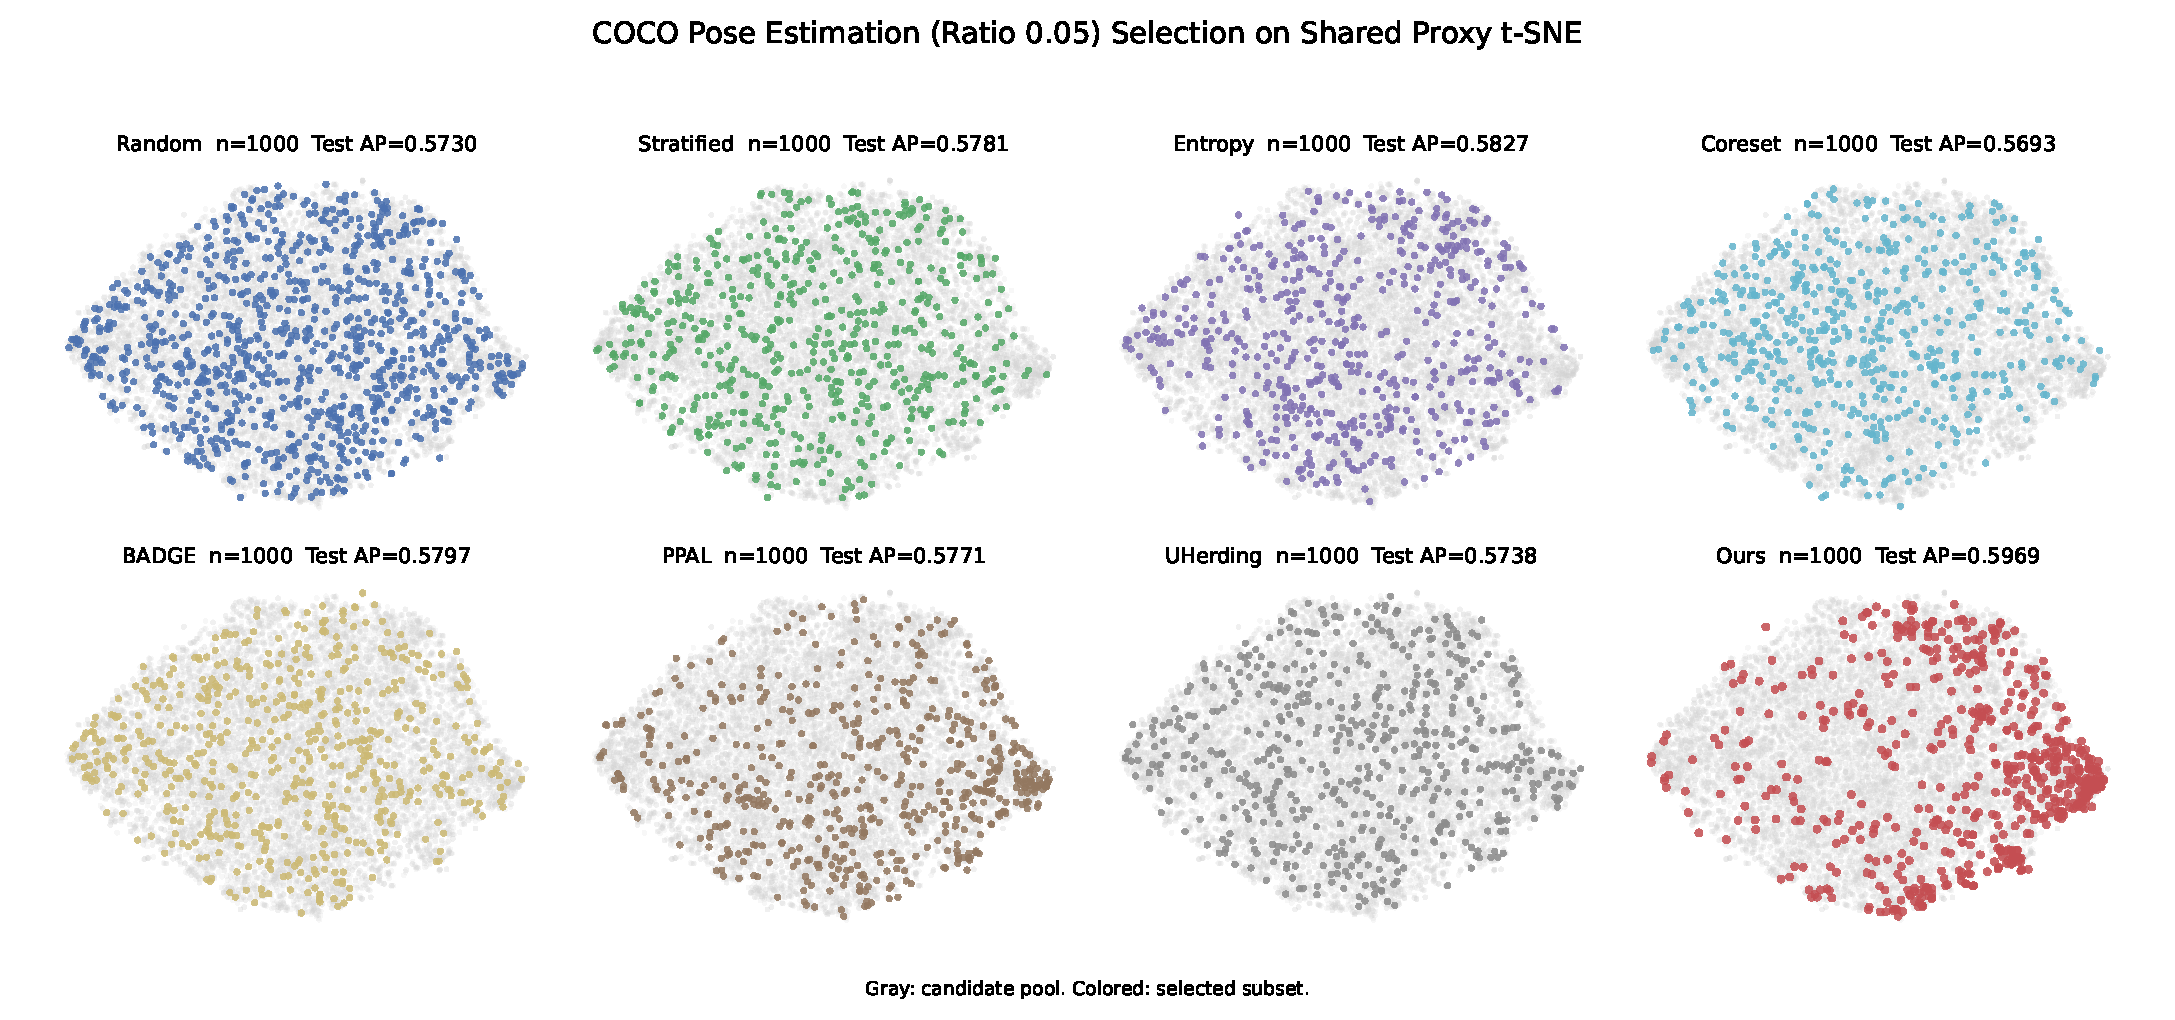
\includegraphics[width=\linewidth]{figures/ratio0p05_selection_tsne/coco_brown_rainy_ratio0p05_selection_tsne.pdf}
\caption{COCO pose-estimation ratio-$0.05$ selected subsets visualized on a shared source-image t-SNE embedding ($n=1{,}000$). Each method selects an identical source budget of $1{,}000$ training images from the $N=20{,}000$ candidate pool. Subpanel titles report downstream test AP values matching the constrained-budget evaluations in Table~\ref{tab:constrained-source-budget}.}
\label{fig:tsne-r005-coco}
\end{figure*}

\begin{figure*}[p]
\centering
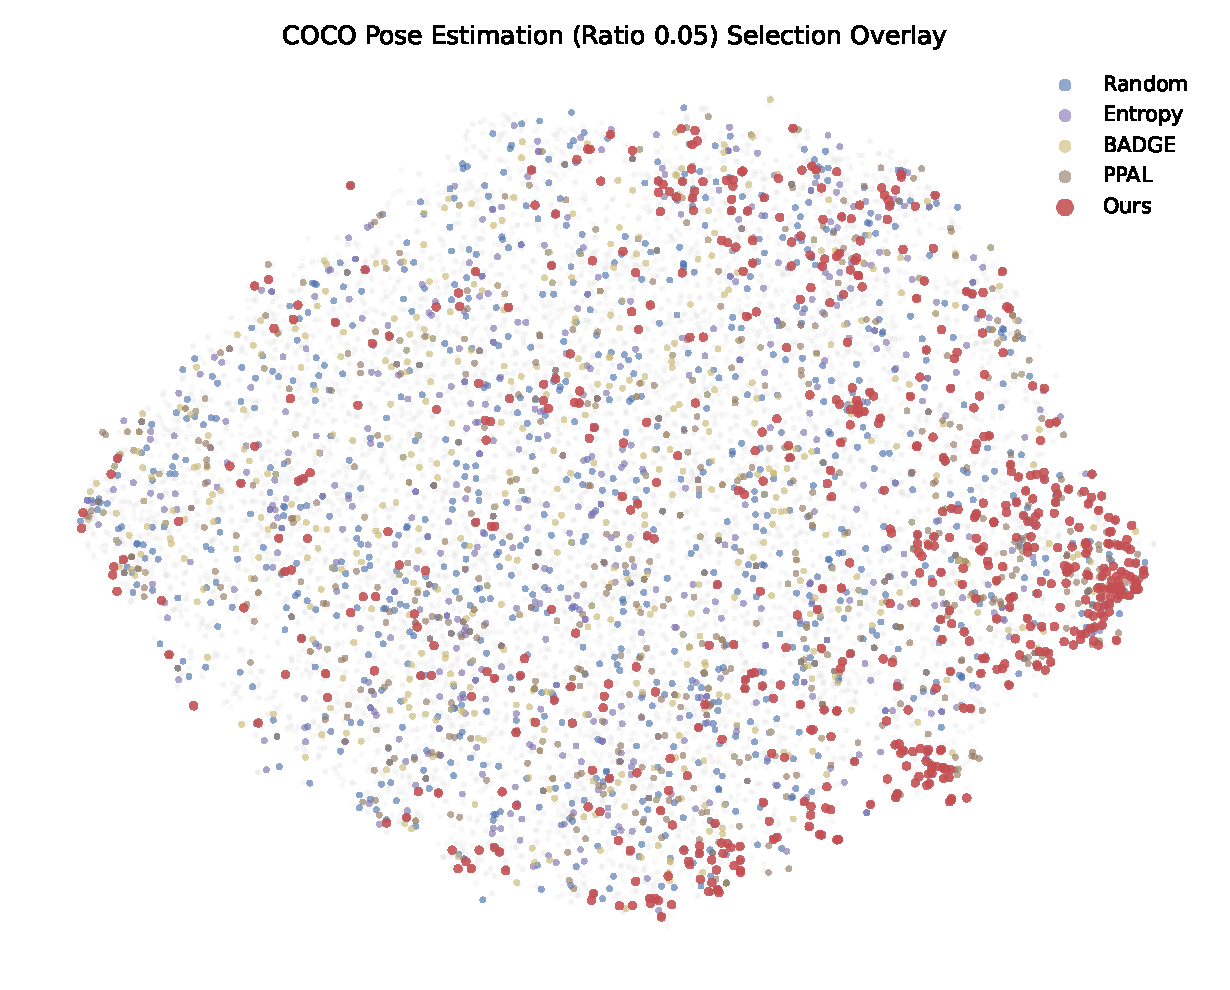
\includegraphics[width=0.86\linewidth]{figures/ratio0p05_selection_tsne/coco_brown_rainy_ratio0p05_selection_tsne_overlay.pdf}
\caption{COCO pose-estimation ratio-$0.05$ overlay view for selected active-learning baselines and \model ($n=1{,}000$).}
\label{fig:tsne-overlay-r005-coco}
\end{figure*}
